%%%%%%%%%%%%%%%%%%%%%%%%%%%%%%%%%%%%%%%%%%%%%%%%%%%%%%%%%%%%%%%
%% KFUPM Thesis Template for MS and PhD Students
%% DO NOT ALTER THE CLASS FILE 'kfupm_thesis.cls'
%%%%%%%%%%%%%%%%%%%%%%%%%%%%%%%%%%%%%%%%%%%%%%%%%%%%%%%%%%%%%%%

%% Choose ONE document class only
\documentclass[ms,twoside,12pt]{kfupm_thesis}
% \documentclass[printready,ms,twoside,12pt]{kfupm_thesis}
% \documentclass[phd,twoside,12pt]{kfupm_thesis}
% \documentclass[printready,phd,twoside,12pt]{kfupm_thesis}

%%%%%%%%%%%%%%%%%%%%%%%%%%%%%%%%%%%%%%%%%%%%%%%%%%%%%%%%%%%%%%%
%% Margin and Text Width Configuration
%%%%%%%%%%%%%%%%%%%%%%%%%%%%%%%%%%%%%%%%%%%%%%%%%%%%%%%%%%%%%%%

\textwidth=5.75in
\oddsidemargin=0.505in

%%%%%%%%%%%%%%%%%%%%%%%%%%%%%%%%%%%%%%%%%%%%%%%%%%%%%%%%%%%%%%%
%% Essential Packages
%%%%%%%%%%%%%%%%%%%%%%%%%%%%%%%%%%%%%%%%%%%%%%%%%%%%%%%%%%%%%%%

\usepackage{graphicx}
\usepackage{latexsym}
\usepackage{amsmath}
\usepackage{epsfig}
\usepackage{amssymb}
\usepackage{mathtools}
\usepackage{mathrsfs}
\usepackage{float}
\usepackage{xfrac}
\usepackage{mhsetup}

\usepackage{lipsum}


%%%%%%%%%%%%%%%%%%%%%%%%%%%%%%%%%%%%%%%%%%%%%%%%%%%%%%%%%%%%%%%
%% Polyglossia for Arabic and English
%%%%%%%%%%%%%%%%%%%%%%%%%%%%%%%%%%%%%%%%%%%%%%%%%%%%%%%%%%%%%%%

\usepackage{polyglossia}
\setmainlanguage{english}


%%%%%%%%%%%%%%%%%%%%%%%%%%%%%%%%%%%%%%%%%%%%%%%%%%%%%%%%%%%%%%%
%% Hyperref Setup
%%%%%%%%%%%%%%%%%%%%%%%%%%%%%%%%%%%%%%%%%%%%%%%%%%%%%%%%%%%%%%%

% Handle polyglossia bug with maketitle
\let\keptmaketitle\maketitle

\usepackage{hyperref}
\hypersetup{
    colorlinks,
    citecolor=blue,
    filecolor=blue,
    linkcolor=black,
    urlcolor=blue
}



%%%%%%%%%%%%%%%%%%%%%%%%%%%%%%%%%%%%%%%%%%%%%%%%%%%%%%%%%%%%%%%
%% Empty Page Between Title and Committee Page (Double-Sided)
%%%%%%%%%%%%%%%%%%%%%%%%%%%%%%%%%%%%%%%%%%%%%%%%%%%%%%%%%%%%%%%
\usepackage{enumitem}

\newcommand{\clearemptydoublepage}{%
  \clearpage
  {\pagestyle{empty}\cleardoublepage}%
}

%%%%%%%%%%%%%%%%%%%%%%%%%%%%%%%%%%%%%%%%%%%%%%%%%%%%%%%%%%%%%%%
%% Bibliography Heading Format
%%%%%%%%%%%%%%%%%%%%%%%%%%%%%%%%%%%%%%%%%%%%%%%%%%%%%%%%%%%%%%%


\addto{\captionsenglish}{%
  \renewcommand{\bibname}{REFERENCES}
}

%%%%%%%%%%%%%%%%%%%%%%%%%%%%%%%%%%%%%%%%%%%%%%%%%%%%%%%%%%%%%%%
%% Figure and Graphics Setup
%%%%%%%%%%%%%%%%%%%%%%%%%%%%%%%%%%%%%%%%%%%%%%%%%%%%%%%%%%%%%%%

\DeclareGraphicsExtensions{.pdf,.png,.jpg,.eps}
\graphicspath{{./figs/}}

%%%%%%%%%%%%%%%%%%%%%%%%%%%%%%%%%%%%%%%%%%%%%%%%%%%%%%%%%%%%%%%
%% Input Path for Class/Bib Files
%%%%%%%%%%%%%%%%%%%%%%%%%%%%%%%%%%%%%%%%%%%%%%%%%%%%%%%%%%%%%%%

\usepackage{import}
\makeatletter
\def\input@path{{./bst/}}
\makeatother

%%%%%%%%%%%%%%%%%%%%%%%%%%%%%%%%%%%%%%%%%%%%%%%%%%%%%%%%%%%%%%%
%% Glossaries for Symbols and Abbreviations
%%%%%%%%%%%%%%%%%%%%%%%%%%%%%%%%%%%%%%%%%%%%%%%%%%%%%%%%%%%%%%%

\usepackage[xindy,toc,acronym,nonumberlist,nopostdot]{glossaries}
\makeglossaries
\renewcommand*{\glsclearpage}{} % remove empty pages before lists

%% Define symbol macro
\newcommand{\sym}[4]{%
    \newglossaryentry{#1}{%
        name={#2},
        description={#3},
        symbol={#2},
        sort={#4}
    }%
}

%% Example symbol definitions
\sym{mysymbol}{\ensuremath{\Gamma}}{This is a symbol}{gamma}
\sym{yoursymbol}{\ensuremath{\Theta}}{This is a symbol}{tetha}



%% Example acronyms
\newacronym{phd}{Ph.D.}{Doctor of Philosophy}
\newacronym{uav}{UAV}{Unmanned Aerial Vehicle}
\newacronym{vrp}{VRP}{Vehicle Routing Problem}

%%%%%%%%%%%%%%%%%%%%%%%%%%%%%%%%%%%%%%%%%%%%%%%%%%%%%%%%%%%%%%%
%% Polyglossia for Arabic and English
%%%%%%%%%%%%%%%%%%%%%%%%%%%%%%%%%%%%%%%%%%%%%%%%%%%%%%%%%%%%%%%

\setotherlanguage{arabic}
\newfontfamily\arabicfont[Script=Arabic]{Scheherazade}
% Arabic font
\let\maketitle\keptmaketitle 

%---------------------------------------------------
%added to overcome the text strecting from top to bottom when using openright
\raggedbottom%

\newcommand{\authorname}{Jimmy Palomino Huilcapi}
%--------------------------------------------------------
\begin{document}
    
    %%%%%%%%%%%%%%%%%%%%%%%%%%%%%%%%%%%%%%%%%%%%%%%%%%%%%%%%%%%%%%%%%%%%%%%%%%%%%
%% Title Page Information
%%%%%%%%%%%%%%%%%%%%%%%%%%%%%%%%%%%%%%%%%%%%%%%%%%%%%%%%%%%%%%%%%%%%%%%%%%%%%

% Title of the Thesis / Dissertation
\title{Your Thesis Title}

% Author's Full Name
\author{Your Name}

% Academic Major (not department unless the same)
\dept{INDUSTRIAL AND SYSTEM ENGINEERING}

% Date of Submission (Month and Year)
\date{DECEMBER 2025}

%%%%%%%%%%%%%%%%%%%%%%%%%%%%%%%%%%%%%%%%%%%%%%%%%%%%%%%%%%%%%%%%%%%%%%%%%%%%%
%% Arabic Abstract Information
%%%%%%%%%%%%%%%%%%%%%%%%%%%%%%%%%%%%%%%%%%%%%%%%%%%%%%%%%%%%%%%%%%%%%%%%%%%%%

\artitle{عنوان الرسالة}          % Title in Arabic
\arname{اسم الطالب}             % Name in Arabic
\ardept{قسم الطلاب}             % Department in Arabic
\ardate{أدخل الشهر والسنة}       % Date in Arabic

%%%%%%%%%%%%%%%%%%%%%%%%%%%%%%%%%%%%%%%%%%%%%%%%%%%%%%%%%%%%%%%%%%%%%%%%%%%%%
%% Title and Committee Pages
%%%%%%%%%%%%%%%%%%%%%%%%%%%%%%%%%%%%%%%%%%%%%%%%%%%%%%%%%%%%%%%%%%%%%%%%%%%%%

\maketitle                      % Generate Title Page

% Advisor (Supervisor)
\adviser{Advisor}

% Co-Advisor (if applicable)
% \coadviser{Dr. [Co-Advisor Name]}

% Committee Members
\memberone{Member 1}
\membertwo{Member 2}
\memberthree{Member 3}
\memberfour{Member 4}

% Department Chairman
\chairman{Chairman}

% Dean of Graduate Studies
\deanGS{Dr. Suliman Al-Homidan}


    %%%%%%%%%%%%%%%%%%%%%%%%%%%%%%%%%%%%%%%%%%%%%%%%%%%%%%%%%%%%%%%%%%%%%%%%%%%%%
%% Committee Page Generation
%%%%%%%%%%%%%%%%%%%%%%%%%%%%%%%%%%%%%%%%%%%%%%%%%%%%%%%%%%%%%%%%%%%%%%%%%%%%%

\clearemptydoublepage           % Insert blank page in double-sided mode
\MakeCommitteeCertificate       % Generate the committee certificate page

% Optional alternatives (not typically required):
% \MakeCertificateThree
% \MakeCertificateFive

\thispagestyle{plain}           % Set page style for this page
    \newpage
\thispagestyle{empty}
\vspace*{\fill}
\begin{center}
{\large {\copyright \authorname  \\
\the\year
}}
\end{center}
\vspace*{\fill}
    \newpage
\topskip0pt
\vspace*{\fill}
\begin{center}
{\large \emph{Dedication}}
\end{center}
\vspace*{\fill}
    \newpage%

\Acknowledgements{
\begin{center}
\noindent \emph{It's customary and good manners to say thank you. Keep in mind that one has to use one's own words when writing an acknowledgement. It's customary and good manners to say thank you. Keep in mind that one has to use one's own words when writing an acknowledgement.}

\emph{It's customary and good manners to say thank you. Keep in mind that one has to use one's own words when writing an acknowledgement. It's customary and good manners to say thank you. Keep in mind that one has to use one's own words when writing an acknowledgement.}
\end{center}
}

    \begin{preamble}
        % \begin{preamble}

%Printing list of symbols and abbreviations
%setting the width of the labels the same as 2.5cm as required by DGS template
\setlist[description]{leftmargin=!, labelwidth=2.5cm, font=\normalfont} %
{
\setstretch{1.5}%
%
\newpage
\phantomsection
\printglossary[title=LIST OF SYMBOLS, toctitle=LIST OF SYMBOLS, nogroupskip] %

%
\newpage%
\phantomsection
\printglossary[title=LIST OF ABBREVIATIONS, toctitle=LIST OF ABBREVIATIONS,type=\acronymtype,nogroupskip] %
\setstretch{2}%
}
\setlist[description]{style=standard} %
%
% The following file defines the Thesis abstract
\textwidth=5.75in
\oddsidemargin=0.505in


% \end{preamble}


        
        
\newpage

%% Please enter the Complete Abstract in the following in place of xxxxx.

\Abstract{
\emph{When writing an abstract, bare in mind an abstract is a short descriptive summary of your thesis. The number of words accepted might vary e.g. $200-250$ words. An MS thesis abstract need not exceed two pages. Abstracts are typically written last although they are the most important part of the thesis. They should have a little bit of everything: the background, the scope of your project, the purpose, findings and conclusions. An abstract is neither paragraphed nor cited. It should not be written as a literature review or a discussion of results. In a simplistic manner, your abstract, in a few words, should answer the questions: why should one care about your research; how did you get your results; what did you learn, find, create, invent; and finally what do your results imply?}
}



        \newpage
\AbstractArabic{ %
عند كتابة ملخص ، ضع في اعتبارك مجرد ملخص هو ملخص وصفي قصير لأطروحتك. قد يختلف عدد الكلمات المقبولة على سبيل المثال:
\LR { $ 250-200 $ }   
كلمة. يجب ألا يتعدى ملخص رسالة ماجستير صفحتين. عادة ما يتم كتابة الملخصات على الرغم من كونها أهم جزء في الرسالة. يجب أن يكون لديهم القليل من كل شيء: الخلفية ، نطاق مشروعك ، الغرض ، النتائج والاستنتاجات. الملخص ليس مفصولًا أو مذكورًا. لا ينبغي أن تكون مكتوبة كمراجعة للأدبيات أو مناقشة النتائج. بطريقة مبسطة ، يجب أن يجيب الملخص الخاص بك ، في كلمات قليلة ، على الأسئلة: لماذا يجب أن يهتم المرء بأبحاثك ؛ كيف حصلت على نتائجك؟ ماذا تعلمت ، وجدت ، وخلقت ، وأخيرًا ماذا تعني نتائجك؟
\\
%\LR{Use LR command to write english words or RL for sentences in the arabic text}
} %
    \end{preamble}

    \chapter{Introduction}

\section{Background and Motivation}
\lipsum[1-2]

\section{Problem Statement}
\lipsum[3]

\section{Objectives of the Thesis}
\begin{itemize}
    \item To develop a robust finite element model for the LSPPMSM under healthy and faulty conditions.
    \item To simulate inter-turn short-circuit faults and extract key diagnostic features.
    \item To evaluate the effectiveness of frequency-domain and time-frequency analyses.
\end{itemize}
\lipsum[4]

\section{Scope and Limitations}
\lipsum[5]

\section{Thesis Organisation}
This thesis is organised as follows:
\begin{itemize}
    \item \textbf{Chapter 1} introduces the background, problem statement, objectives, and organisation.
    \item \textbf{Chapter 2} presents a comprehensive literature review on FEM-based fault modelling.
    \item \textbf{Chapter 3} details the finite element modelling approach in ANSYS Maxwell.
    \item \textbf{Chapter 4} discusses the simulation of ITSC faults and extraction of current/voltage harmonics.
    \item \textbf{Chapter 5} concludes the findings and outlines recommendations for future work.
\end{itemize}
\lipsum[6]

    \chapter{Literature Review}

\section{Introduction}
The application of finite element method (FEM) to fault diagnosis in permanent magnet synchronous motors (PMSMs) has grown significantly in the past two decades. This chapter reviews key contributions to FEM-based modelling, inter-turn short-circuit (ITSC) fault simulation, and electromagnetic analysis for diagnostic feature extraction.

\section{FEM-Based Modelling of PMSMs}
Several studies have employed FEM to model PMSMs under both healthy and faulty conditions. For example, the authors in \cite{Smith2020} developed a 2D time-stepped transient FEM model to analyse torque ripple and magnetic flux variations due to stator faults. Similarly, \cite{Lee2019} extended the analysis to 3D models, capturing axial effects and end-winding influences.

\section{Simulation of ITSC Faults}
ITSC faults are among the most common incipient failures in PMSMs. Faults are typically introduced in FEM by shorting turns within a stator coil and assigning a small fault resistance \cite{Wang2018}. This approach allows for accurate electromagnetic behaviour prediction during the fault event. The impact of fault location, resistance, and turn percentage has been extensively explored in \cite{Ahmed2022} and \cite{Zhou2021}.

\section{Electromagnetic Quantities for Fault Analysis}
Electromagnetic quantities such as phase currents, back-EMF, and air-gap flux density are crucial for identifying ITSC faults. Spectral and time-frequency analyses on current signals have shown promise in detecting early-stage faults \cite{Khan2021}. Additionally, circulating currents between parallel paths have been proposed as indicators of asymmetry \cite{Chen2023}.

\section{Limitations in Existing Literature}
Most FEM studies assume linear material properties and ideal winding configurations. Moreover, temperature dependence and saturation effects are often neglected. Some works like \cite{Patel2020} attempt to address these through multi-physics co-simulation, but at the cost of increased computational burden.

\section{Summary}
This review highlights the importance of FEM as a virtual testbench for fault analysis in PMSMs. Although existing literature provides a strong foundation, there remains a need for scalable, fault-inclusive FEM models with realistic winding, resistance, and control conditions tailored to inverter-fed operations.


    \chapter{Methodology}

\section{Overview}
This chapter outlines the methodology adopted in this study. It includes system modelling, the use of glossary terms such as \gls{mysymbol} and \gls{yoursymbol}, and utilises acronyms such as \gls{phd}. Once the acronym has been introduced, it appears simply as \gls{phd}. For completeness, \acrfull{phd}, \acrshort{phd}, and \glspl{phd} are also demonstrated.

\section{System Model and Notation}
{Enter the material. The symbols and abbreviations defined can be used using the \textbackslash gls command. The defined symbol is \gls{mysymbol} and \gls{yoursymbol}. When the acronym is used for the first time it gives the full form as follows \gls{phd}. Thereafter, it only gives the abbreviation as follows \gls{phd}. The full form, short form and plural of the acronym can be called as follows \acrfull{phd}, \acrshort{phd} and \glspl{phd} respectively.}

\section{Example Figure}
\begin{figure}[!ht]
\centering
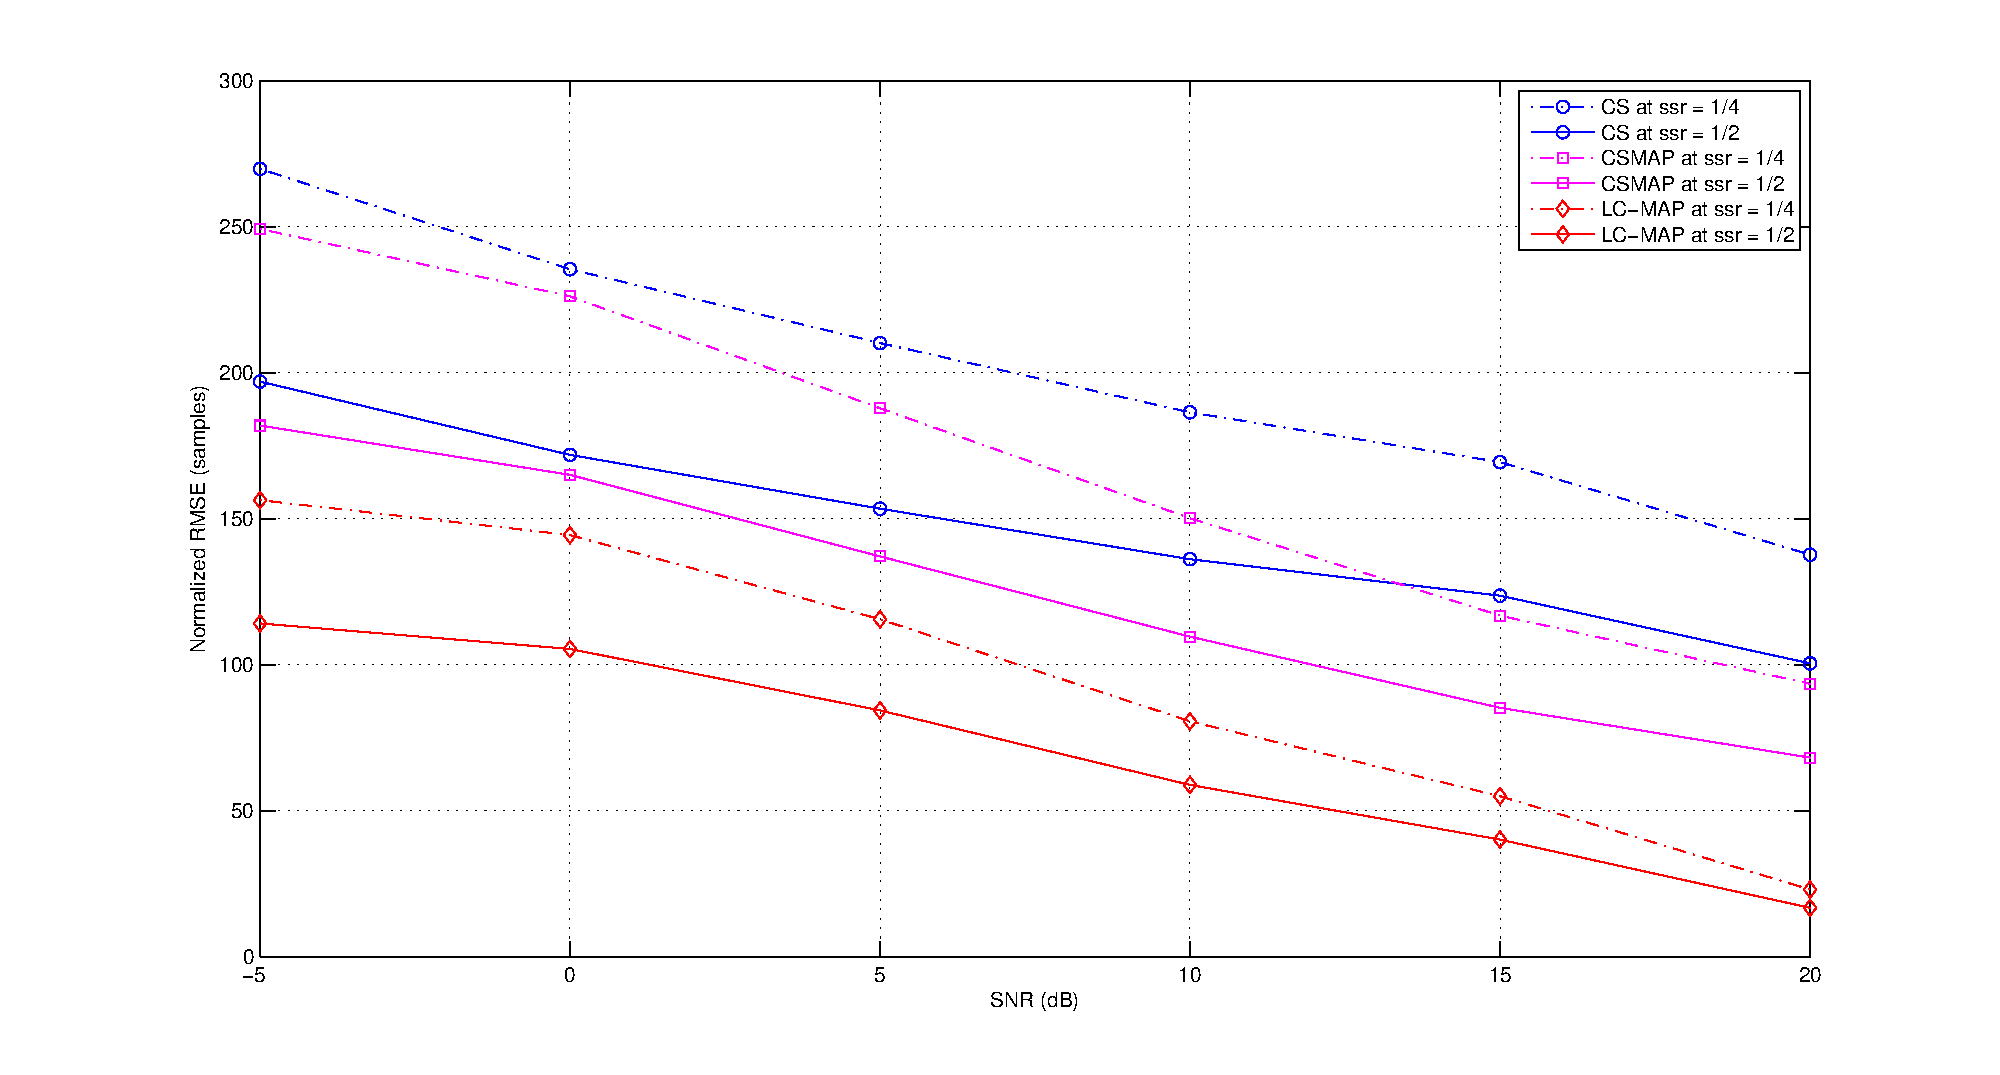
\includegraphics[width=7.5cm, height=5.26cm]{Images/plot.pdf}
\caption{This is a plot to show the results.}
\label{fig:Plot}
\end{figure}

\section{Mathematical Formulation}
{Enter material \cite{Zhang2004}.}

\begin{align}
\label{eq:TimeModel2a}
r(n \delta) &= \sum_{l=0}^{L-1} a_l \, \mathit{g}(\delta - m_l \delta) + \omega(n \delta)
\end{align}

The sub-sampled signal $\mathbf{y}$ at the receiver can be represented in matrix form as:

\begin{equation}
\label{eq:LinModel01}
\mathbf{y} = \mathbf{G} \mathbf{a} + \boldsymbol{\omega}
\end{equation}

where

\begin{equation}
\label{eq:P}
\mathbf{G} = \left[
\begin{matrix}
\mathit{g}(n - m_0) & \cdots & \mathit{g}(n - m_N) \\
\mathit{g}(n + \mu - m_1) & \cdots & \mathit{g}(n + 1 - m_N) \\
\vdots & \ddots & \vdots \\
\mathit{g}(n + \mu - m_M) & \cdots & \mathit{g}(n + \frac{M-1}{\mu} - m_N)
\end{matrix}
\right]
\end{equation}

\section{Additional Section}
{Enter material \cite{Tesi2006}.}

\section{Another Section}
{Enter material \cite{Gezici2009}.}

\subsection{Sub-Section Title}
{Sub-section.}

\subsection{Sub-Sub-Section Title}
{Sub-section \cite{Carbonelli2003}.}

\section{Supplementary Material}
{Enter material \cite{Bajwa2010b}.}

\section{Example Table}

\begin{table}[!ht]
\centering
\begin{tabular}{|c|c|c|c|c|c|c|}
\hline
Itr. No. & $\boldsymbol \Theta_n$ & Size of $\underline{\boldsymbol \alpha}_i$ & \multicolumn{4}{c|}{Residual: $r_i^n = \Vert \mathbf{y} \Vert_{\boldsymbol \Sigma_i}^{2}$} \\ \cline{4-7}
$(n)$ & $(L \times n)$ & $(n \times 1)$ & $i=1$ & $i=2$ & \dots \dots & $i=C$ \\
\hline
1 & $\boldsymbol \Theta_1 = [\boldsymbol \theta_1]$ & $(1 \times 1)$ & $r_1^1$ & $r_2^1$ & \dots \dots & $r_C^1$ \\
\hline
2 & $\boldsymbol \Theta_2 = [\boldsymbol \Theta_1 \boldsymbol \theta_2]$ & $(2 \times 1)$ & $r_1^2$ & $r_2^2$ & \dots \dots & $r_C^2$ \\
\hline
3 & $\boldsymbol \Theta_3 = [\boldsymbol \Theta_2 \boldsymbol \theta_3]$ & $(3 \times 1)$ & $r_1^3$ & $r_2^3$ & \dots \dots & $r_C^3$ \\
\hline
\vdots & \vdots & \vdots & \vdots & \vdots & \dots \dots & \vdots \\
\hline
$L-1$ & $\boldsymbol \Theta_{L-1} = [\boldsymbol \Theta_{L-2} \boldsymbol \theta_{L-1}]$ & $((L-1) \times 1)$ & $r_1^{L-1}$ & $r_2^{L-1}$ & \dots \dots & $r_C^{L-1}$ \\
\hline
$L$ & $\boldsymbol \Theta_L = [\boldsymbol \Theta_{L-1} \boldsymbol \theta_L]$ & $(L \times 1)$ & $r_1^L$ & $r_2^L$ & \dots \dots & $r_C^L$ \\
\hline
\end{tabular}
\caption{This is a Table.}
\label{tab:Table}
\end{table}


    \appendix
    \chapter{Proofs} %Appendix A

    \chapter{Supplementary Material} %Appendix B


    \bibliographystyle{IEEEtran}
    \bibliography{Body/3.References}

    \chapter*{Vitae}
\addcontentsline{toc}{chapter}{Vitae}

\noindent
\textbf{Name:} Jimmy Palomino Huilcapi \\
\textbf{Nationality:} Ecuadorian \\
\textbf{Date of Birth:} February 11, 1998 \\
\textbf{Email:} jimmy.palomino@yahoo.com \\
\textbf{Address:} Dhahran, Eastern Province, Saudi Arabia \\

\vspace{1em}
\noindent
\textbf{Academic Background:}
\begin{itemize}
    \item Bachelor of Science in Electrical Engineering from Escuela Superior Politécnica del Litoral (ESPOL), Ecuador, 2021.
    \item Master of Science in Electrical Engineering from King Fahd University of Petroleum and Minerals (KFUPM), Saudi Arabia, 2025 (expected).
\end{itemize}

\vspace{1em}
\noindent
\textbf{Professional Experience:}
\begin{itemize}
    \item \textbf{Academic Assistant} at KFUPM – Lab instruction, grading, and teaching support (2023–Present).
    \item \textbf{Academic Ambassador} at KFUPM – Promoted graduate programs in Latin America (2023–Present).
    \item \textbf{Academic Assistant in Electrical Machines} at ESPOL – Lab support and motor/generator testing (2020–2021).
\end{itemize}


\vspace{1em}
\noindent
\textbf{Languages:}
\begin{itemize}
    \item Spanish – Native or bilingual proficiency
    \item English – Professional working proficiency
\end{itemize}


\end{document}
